\section{Übersicht Immaterialgüterrecht}
\begin{figure}[H]
	\centering
	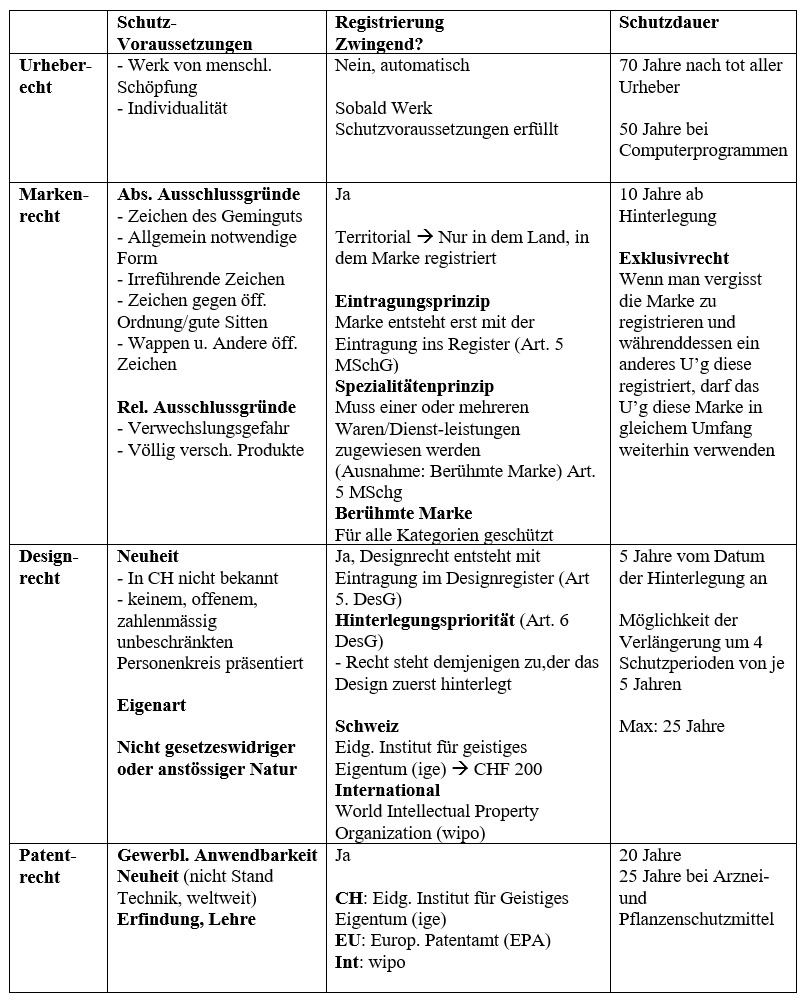
\includegraphics[width=\textwidth]{figures/overviewImaterialgueter.jpeg}
\end{figure}

\section{Gesetzesartikel}

\subsection{Urheberrechtsgesetze (URG)}

\begin{description}
	\tightlist
	\item[Art. 3 URG] Werke zweiter Hand.
	(Siehe \autopageref{sec:Urheberrecht-Schutzvoraussetzugen})

	\item[Art. 6 URG] Als \textbf{Urheber} gilt die \textbf{natürliche Person},
	die das Werk geschaffen hat (\textbf{Schöpferprinzip}).
	(Siehe \autopageref{sec:Urheberrecht-UrheberschaftMiturheberschaft})

	\item[Art. 9.1 URG] Recht auf Erstveröffentlichung
	(Siehe \autopageref{sec:Urheberrecht-Urherberpersönlichkeitsrechte})

	\item[Art. 9.2 URG] Recht auf Anerkennung der Urheberschaft
	(Siehe \autopageref{sec:Urheberrecht-Urherberpersönlichkeitsrechte})

	\item[Art. 11 URG] Recht auf Werkintegrität
	(Siehe \autopageref{sec:Urheberrecht-Urherberpersönlichkeitsrechte})
	
	\item[Art. 16.1 URG] Die Urheberpersönlichkeitsrechte sind unter Lebenden
	nicht übertragbar, von Todes wegen gehen sie jedoch auf die Erben über.
	(Siehe \autopageref{ec:Urheberrecht-Rechtsübergang})

	\item[Art. 17 URG] Automatische Urheberrechtsübertretung bei
	Computerprogrammen die im Rahmen eines Arbeitsvertrages zustande gekommen
	ist.
	(Siehe \autopageref{sec:Urheberrecht-AbhängigeWerkschöpfung})
	
	\item[Art. 19 URG] Grenzen/Schranken des Urheberrechts
	(Siehe \autopageref{sec:Urheberrecht-Schranken})
\end{description}

\subsection{Datenschutz}

\begin{description}
	\tightlist
	\item[Art. 26 ArGV 3] Überwachung des Arbeitnehmenden
	(Siehe \autopageref{sec:IW-Überwachung}) 

	\item[Art. 2 DSG] Geltungsbereich Datenschutzgesetz
	(Siehe \autopageref{sec:Datenschutz-Geltungsbereich})
	
	\item[Art. 3 DSG] Begriffe und Definitionen im DSG
	(Siehe \autopageref{sec:Datenschutz-Begriffe})

	\item[Art. 4 DSG] Datenschutzgrundsätze
	(Siehe \autopageref{sec:Datenschutz-Datenschutzgrundsätze})

	\item[Art. 5 DSG] Verpflichtung richtigkeit der Daten zu prüfen
	(Siehe \autopageref{sec:Datenschutz-Richtigkeit})

	\item[Art. 6 DSG] Grenzüberschreitende bekanntgabe personenbezogenen
	Daten.
	(Siehe \autopageref{sec:Datenschutz-Grenzübergreifend})

	\item[Art. 7 DSG] Daten müssen technisch gesichert werden
	(Siehe \autopageref{sec:Datenschutz-Datensicherheit})

	\item[Art. 8 DSG] Auskunftsrecht über die gesamelten Daten
	(Siehe \autopageref{sec:Datenschutz-Auskunftsrecht})

	\item[Art. 10A DSG] Datenverabrietung durch Dritte
	(Siehe \autopageref{sec:Datenschutz-Dritte})

	\item[Art. 14 DSG] Beim Sammeln besonders schützenswerten
	Personendaten müssen die Personen infomriert weren.
	(Siehe \autopageref{sec:Datenschutz-Informationspflicht})

	\item[Art. 34 DSG] Strafen im Bezug auf Datenschutzverletzungen
	(Siehe \autopageref{sec:Datenschutz-Strafe})

	\item[Art. 35 DSG] Verletzung der beruflichen Schweigepflicht
	(Siehe \autopageref{sec:Datenschutz-Schweigepflicht})

	\item[Art. 28 ZGB] Schutz der Persönlichkeit.
	(Siehe \autopageref{sec:Datenschutz-SchutzPersönlichkeit})

	\item[Art. 328B OR] Datenschutz im Arbeitsverhältnis
	(Siehe \autopageref{sec:Datenschutz-Arbetsverhältnis}) 
\end{description}

\subsection{Digitale Geschäftsführung (Digitale Transformation)}
\begin{description}
	\tightlist
	\item[Art. 3 GeBüV] Geschäftsbücher müssen integer aufbewahrt
	werden. (Siehe \autopageref{sec:DigiTrans-Integrität})

	\item[Art. 4 GeBüV] Dokumentationspflicht
	(Siehe \autopageref{sec:DigiTrans-Dokumentationspflicht})

	\item[Art. 754 OR] Haftung der Verwaltung (VR)
	(Siehe \autopageref{sec:DigiTrans-VR})

	\item[Art. 958f OR] Aufbewahrungspflichten von Geschäfts- und
	Revisorenbericht.
	(Siehe \autopageref{sec:DigiTrans-Aufbewahrungspflichten})

	\item[Art. 166 StGB] Verpflichtung Führung der Geschäftsbücher. 
	(Siehe \autopageref{sec:DigiTrans-Strafrecht})

	\item[Art. 525 StGB] Verpflichtung zur odrdnungsgemäser Führung
	der Geschäftsbücher. 
	(Siehe \autopageref{sec:DigiTrans-Strafrecht})
\end{description}

\subsection{Whistleblowing}
\begin{description}
	\tightlist
	\item[Art. 10 EMRK \& Art. 16] Recht auf freie Meinungsäusserung
	(Siehe \autopageref{sec:IW-Schutz}) 

	\item[Art. 22a BPG] Beamte sind verpflichtet illegale Aktivitäten
	zu melden 
	(Siehe \autopageref{sec:IW-Verpflichtungen})

	\item[Art. 321a Abs. 1 OR] Treuepflichten: Illegale Aktivitäten
	müssen dem Vorgesetzten gemeldet werden. 
	(Siehe \autopageref{sec:IW-Verpflichtungen})

	\item[Art. 336 OR] Rechtlicher Schutz auf missbräuchliche Kündigung
	im Falle von Whistleblowing. 
	(Siehe \autopageref{sec:IW-Schutz}) 

	\item[Art. 716a Abs. 1 OR] Corporate Governance \& Compliance/Risk
	Management verlangen ständige Sicherheitsüberprüfungen
	(Siehe \autopageref{sec:IW-Verpflichtungen})
\end{description}

\subsection{Cyber-Delikte}
\begin{description}
	\tightlist
	\item[Art. 143 StGB] Unbefugte Datenbeschaffung
	(Siehe \autopageref{sec:CD-Datenbeschaffung})

	\item[Art. 143bis StGB] Unbefugte Eindringen in eine
	Datenverarbeitungsanlage
	(Siehe \autopageref{sec:CD-Eindringen})

	\item[Art. 144bis StGB] Datenbeschädigung
	(Siehe \autopageref{sec:CD-Datenbeschädigung})

	\item[Art. 147 StGB] Betrügerischer Missbrauch einer
	Datenverarbeitungsanlage
	(Siehe \autopageref{sec:CD-Missbrauch})

	\item[Art. 150bis StGB] Herstellen \& Inverkehrbringen von
	Materialien zur unbefugten Entschlüsselung codierter Angebote
	(Siehe \autopageref{sec:CD-Herstellen})

	\item[Art. 162 StGB] Verletzung des Fabrikations- oder
	Geschäftsgeheimnisses
	(Siehe \autopageref{sec:CD-Overview})

	\item[Art. 173 StGB] Üble Nachrede
	(Siehe \autopageref{sec:CD-Ehrverletzung})
 
	\item[Art. 174 StGB] Verleumdung
	(Siehe \autopageref{sec:CD-Ehrverletzung})

	\item[Art. 177 StGB] Beschimpfung
	\item[(Siehe \autopageref{sec:CD-Ehrverletzung})] 

	\item[Art. 179 StGB] Verletzung des Schriftgeheimnisses
	(Siehe \autopageref{sec:CD-Overview})
 
	\item[Art. 179novies StGB] Unbefugtes Beschaffen von Personendaten
	(Siehe \autopageref{sec:CD-Overview})

	\item[Art. 197 StGB] Pornografie
	(Siehe \autopageref{sec:CD-Overview})

	\item[Art. 239 StGB] Störung von Betrieben, die der
	Allgemeinheit dienen
	(Siehe \autopageref{sec:CD-Overview})

	\item[Art. 261bis StGB] Rassendiskriminierung
	(Siehe \autopageref{sec:CD-Overview})
 
	\item[Art. 273 StGB] Wirtschaftlicher Nachrichtendienst
	(Siehe \autopageref{sec:CD-Overview}) 
\end{description}

\subsection{Verträge auf Arbeitsleistung}
\begin{description}
	\tightlist
	\item[Art. 363 OR] Pflicht zur Herstellung eines Werkes im
	Werkvertrag sowie dessen Bezahlung.
	(Siehe \autopageref{sec:Werkvertrag-RechtePflichten}) 
  
	\item[Art. 366 Abs. 2 OR] Mängelrecht: Ersatzvornahme
	(Siehe \autopageref{sec:Werkvertrag-Mängelrechte})

	\item[Art. 367 OR] Pflicht zur Lieferung eines Werkes im
	Werkvertrag.
	(Siehe \autopageref{sec:Werkvertrag-RechtePflichten}) 

	\item[Art. 368] Mängelrechte: Minerung, Nachbesserung und Wandelung
	(Siehe \autopageref{sec:Werkvertrag-Mängelrechte})

	\item[Art. 370 OR] Pflicht zur Abnahme eines Werkes welches im Rahmen
	eines Werkvertrages erstellt wurde.
	(Siehe \autopageref{sec:Werkvertrag-RechtePflichten}) 

	\item[Art. 372 OR] Pflicht zur bezahlung eines hergestellten Werkes.
	(Siehe \autopageref{sec:Werkvertrag-RechtePflichten}) 

	\item[Art. 373 OR] Vereinbarter Preis bei Werkvertrag
	(Siehe \autopageref{sec:Werkvertrag-Preisvereinbarung})

	\item[Art. 374 OR] Fehlende Preisvereinbarung bei Werkvertrag
	(Siehe \autopageref{sec:Werkvertrag-Preisvereinbarung}) 
 
	\item[Art. 404 OR] Kündigungsrecht bei Auftrag
	(Siehe \autopageref{sec:Auftrag-Overview})  
\end{description}

\subsection{Markenschutzrecht}
\begin{description}
	\tightlist
	\item[Art. 5 MSchG] Eintragungsprinzip: Marke entsteht erst mit der
	Eintragung ins Register.
	(Siehe \autopageref{sec:Markenrecht-Registrierung})
	\item[Art. 6 MSchG] Hiterlegungspriorität. Wer die Marke zuerst hinterlegt
	hat die Rechte.
	(Siehe \autopageref{sec:Markenrecht-Registrierung})
	\item[Art. 15 MSchG] Bisheriger Gebrauch einer Marken kann durch
	Registrierung nicht verboten werden.
	(Siehe \autopageref{sec:Markenrecht-Registrierung})
	\item[Art. 15 MSchG] Ausnahme zum Eintragungsprinzip ist die
	\textbf{bekannte Marke}.
	(Siehe \autopageref{sec:Markenrecht-Registrierung})
\end{description}

\subsection{Design-/Patentrecht}
\begin{description}
	\tightlist
	\item[Art. 1 DesG] Definition Design
	(Siehe \autopageref{sec:Designrecht-Grundlage})

	\item[Art. 5 DesG] Entstehung des Designrechts
	(Siehe \autopageref{sec:Designrecht-Registrierung})

	\item[Art. 6 DesG] Hiterlegungspriorität.\\
	(Siehe \autopageref{sec:Designrecht-Hinterlegungsprioritaet})

	\item[Art. 1 PatG] Zweck des Patentrecht
	(Siehe \autopageref{sec:Patentrecht-Zweck})

	\item[Art. 7 Abs. 2] Nicht patentberechtigt sind Dinge, die sich aus dem
	Stand der Technik ergeben.
	(Siehe \autopageref{sec:Patentrecht-Rechtsgrundlage})

	\item[Art. 8 PatG] Verbot zur Benutzung einer patentierten Erfindung.\\
	(Siehe \autopageref{sec:Patentrecht-Zweck})

	\item[Art. 9 PatG] Begrenzug der Schutzwirkung für private, Forschungs-
	und Unterrichtszwecke.\\
	(Siehe \autopageref{sec:Patentrecht-Begrenzug})

	\item[Art. 322 OR] Diensterfindung und Gelegenheitserfindung.
	(Siehe \autopageref{sec:Patentrecht-Arbeitnehmererfindungen})
\end{description}

\subsection{Haftpflichtrecht}
\begin{description}
	\tightlist
	\item[Art. 41 OR] Verschuldungshaftung
	(Siehe \autopageref{sec:Haftpflicht-Arten})

	\item[Art. 52.1 OR] Rechtfertigungsgrund: Notwehr
	(Siehe \autopageref{sec:Haftpflichtrecht-Rechtfertigung})

	\item[Art. 52.2 OR] Rechtfertigungsgrund: Notstand
	(Siehe \autopageref{sec:Haftpflichtrecht-Rechtfertigung})

	\item[Art. 52.3 OR] Rechtfertigungsgrund: Selbsthilfe
	(Siehe \autopageref{sec:Haftpflichtrecht-Rechtfertigung})

	\item[Art. 55 OR OR] Geschäftsherrenhaftung
	(Siehe \autopageref{sec:Haftpflicht-Arten})

	\item[Art. 58 OR OR] Werkeigentümerhaftung/Kausalhaftung
	(Siehe \autopageref{sec:Haftpflicht-Arten})

	\item[Art. 58.1 SVG] Beispiel Gefährdungshaftung im
	Strassenverkehr.
	(Siehe \autopageref{sec:Haftpflicht-Gefaerdungshaftung})

	\item[Art. 679 ZGB] Haftung des Grundeigentümers
	(Siehe \autopageref{sec:Haftpflicht-Arten})
\end{description}

\subsection{Risikomanagement und Versicherungen}
\begin{description}
	\tightlist
	\item[Art. 100 OR] Haftungsbegrenzung
	(Siehe \autopageref{sec:RisikoMgmt-Haftungsbrgrenzungen})

	\item[Art. 717 OR] Sorgfalts- und Treuepflicht der Geschäftsführung/
	Verwaltungsrat.
	(Siehe \autopageref{sec:RisikoMgmt-SorfaltTreuePflicht})

	\item[Art. 754 OR] Haftung für Verwaltung, Geschäftsführung und Liquidation.
	(Siehe \autopageref{sec:RisikoMgmt-HaftungVerwaltung})
\end{description}

\subsection{Öffentlichkeitsrecht und Open Data}
\begin{description}
	\tightlist
	\item[Art. 2 BGÖ] Geltungsbereich: Institutionen.
	(Siehe \autopageref{sec:BGO-Geltungsbereich})

	\item[Art. 5 BGÖ] Geltungsbereich: Betroffene Dokumente.
	(Siehe \autopageref{sec:BGO-Geltungsbereich})

	\item[Art. 7 BGÖ] Ausnahmen des BGÖ.
	(Siehe \autopageref{sec:BGO-Ausnahmen})

	\item[Art. 6 BGÖ] Interessenabwägung zwischen Schutz der
	Privatsphäre und öffentlichem Interesse.
	(Siehe \autopageref{sec:BGO-Intressenabwaegung})
\end{description}

\section{Beispiele}

\subsection{Datenschutz}

\subsubsection{Ist das zulässig?}

\textbf{Anonyme Mitarbeiterbefragung mit Altersangabe. 2 Personen im
Team sind 55 plus.}\\
Nein. Die anonymen Daten dürfen nicht auf Personen zurückverfolgt werden
können.

\mbox{}\\
\textbf{Die Personendaten werden verarbeitet: a) Deutschland, b) in den
USA und c) in der Türkei}

\begin{enumerate}
	\tightlist
	\item Deutschland hat ein vergleichbaren Datenschutzgesetz, also is OK. Die
	europäische Datenschutzrichtlinien sind sogar noch härter.
	\item Die USA hat kein vergleichbares Datenschutzgesetz, also NICHT OK.
	\item Aktuell ist die Situation nicht so, dass sie ein vergleichbares
	Datenschutzgesetz haben. Die Übergabe ist nicht grundsätzlich
	verboten, aber Sie müssen sicherstellen, dass die Daten sicher sind
	(Verträge mit Bearbeitern).
\end{enumerate}

\textbf{Mietgesuch: in einem Feld muss der Mietinteressent sein
Einkommen und Vermögen angeben. Auch das seiner PartnerIn und/oder
Eltern.}\\
Die Frage ist völlig unverhältnismässig und nicht gerechtfertigt.
Ausserdem dürfen persönliche Daten von Dritten nicht ohne Einwilligung
weitergeben.

\mbox{}\\
\textbf{Medizinische Angaben bei Kassenwechsel: Sie müssen ihre
Krankheiten/Unfälle seit der Kindheit bis heute angeben und solche in
ihrer Familie.}\\
Die Daten von Dritten dürfen nicht ohne Einwilligung weitergegeben
werden.

\mbox{}\\
\textbf{Eine Konsumentenschutzorganisation veröffentlicht eine Karte,
auf der die Positionen von GSM/4G-Antennen \& ihre Eigentümer
eingezeichnet sind.}\\
Auch wenn die Eigentümer grösstenteils Swisscom ist, ist das nicht
zulässig. Swisscom ist eine juristische Person und unterliegt auch dem
Datenschutzgesetz.

\mbox{}\\
\textbf{An einem Montagmorgen fordert der Vorgesetzte einer Krankenkasse
alle Lehrlinge auf, eine Urinprobe abzugeben. Er möchte so feststellen,
ob über das Wochenende THC oder andere Rauschmittel konsumiert wurde.}\\
Eine personenbezogene Auswertung ist nicht zulässig. Eine andere
Situation ist es, wenn es sich z.B. um einen Pilot, einen Zugführer oder
einen Arzt handelt.

\mbox{}\\
\textbf{STRAVA oder RUNTASTIC verkaufen ihre Userdaten einer
Versicherung.} Dies ist natürlich nicht erlaubt, sofern es sich um
personenbezogene Daten handelt. In den AGBs darf jedoch eine
anonymisierte Weitergabe festgelegt werden.

\subsubsection{Auskunftsrecht}

\textbf{Wie gehen Sie vor, um Auskunft über Ihre persönlichen Daten zu
erhalten?}\\
Ich muss nur Anfragen und mich ausweisen können. Die Informationen
sollten innerhalb von 30 Tagen kommen. Die Auskunft ist gratis, ausser
es wurde voraus bereits bekundet, dass die Auskunft sehr aufwändig ist
(Kann dann bis zu 300 CHF kosten).

\mbox{}\\
\textbf{Welche Informationen erhalten Sie?}\\
Alle Daten die mit mir in Verbindung stehen.

\mbox{}\\
\textbf{Wie gehen Sie vor, wenn Sie vom Dateninhaber keine Antwort
erhalten?}\\
Klagen.

\subsection{Markenschutzrecht}

\textbf{Ausgangslage:} George importiert aus Thailand einige gefälschte
Marken-Uhren, um diese seinen Kollegen zu schenken. Als das Gold auf der
einen Uhr abzublättern beginnt, bringt er diese zum Neuvergolden einem
Bijoutier, welcher die betroffene Uhrenfirma informiert. Diese reicht in
der Folge Strafanzeige ein und stellt den Antrag, die Uhr sei gestützt
auf Art. 68 MSchG einzuziehen und zu vernichten.\\
\\
\textbf{Kann sich George mit Erfolg dagegen wehren?}\\
Innerhalb der Schweiz ist es nicht verboten, diese gefälschten Artikel
zu privaten Zwecken (Gebrauch) zu benutzen. Nur bei Import, Export oder
Transport durch die Schweiz kann der Hersteller intervenieren.\\

\textbf{Wie wäre der Fall zu beurteilen, wenn George bereits bei der
Einreise am Flug-hafen Kloten von den Zollbehörden gestoppt worden
wäre?}\\
Dies sind sogenannte Kapilar-Importe (Import von kleinen Mengen
gefälschter Ware). Dies ist verboten!\\

\textbf{Ausgangslage 2:} Ein junges Zürcher Unternehmen bringt ein
alkoholfreies Bier auf den Markt und beantragt beim IGE die Eintragung
des Werbeslogans «Nicht immer, aber immer öfter!». Gegen den Eintrag
erhebt ein deutscher Bierproduzent Widerspruch, der mit dem gleichen
Spruch wirbt und diesen in Deutschland (nicht aber in der Schweiz) als
Marke geschützt hat.\\

\textbf{Wird der Widerspruch Erfolg haben?}\\
Der Kläger müsste innerhalb von 3 Monaten reagieren. Und falls dann der
Spruch notorisch bekannt wäre in der Schweiz, hätte der Wiederspruch
Erfolg. Dies müsste man prüfen.
